\section{Real-world Experiments}
\label{sec:real-world}

This section presents real-world experimental results validating our proposed \ac{REACT} method. The experiments were conducted at the underwater robotics facility of the German Research Center for Artificial Intelligence (DFKI), which features a 23$\times$19$\times$8 meter test basin equipped with a 12-camera Qualisys motion capture system for precise state estimation.

\subsection{Real-world experimental setup}
The experimental platform is a BlueROV2, configured identically to the simulation setup. The test environment consists of a pipe structure with a diameter of 0.7 meters and a length of 2.5 meters, as shown in Fig. \ref{fig:pipe}. Two planning modes, identical to those evaluated in simulation, are tested in this study. The first is \ac{REACT}, which represents the full system incorporating \ac{REACT}. The second is the \ac{CPP} baseline without \ac{REACT}. In both modes, a helical trajectory is given as a reference around the pipe.

\begin{figure}[t]
    \centering
    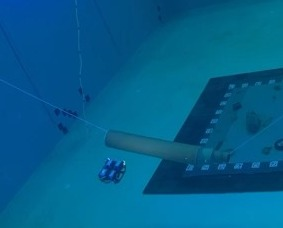
\includegraphics[width=0.65\linewidth]{figures/dfki_pipe.jpeg}
    \caption{ Experimental setup in the DFKI underwater basin showing the BlueROV2 and the test structure. The pipe is suspended horizontally in the water using cables.}
    \label{fig:pipe}
\end{figure}

\subsection{Real-world experimental results}

The real-world tests showed clear benefits of the \ac{REACT} planner compared to the baseline \ac{CPP} approach. Figure~\ref{fig:realworld_trajectory} showed the mission trajectories for both methods.
The baseline \ac{CPP} planner failed to complete the inspection task. At t=124 seconds, the tether became tangled with the pipe structure, stopping the \ac{ROV} and preventing further progress. This resulted in only 80.9\% coverage of the inspection area (Table~\ref{tab:realworld_coverage}).

The proposed \ac{REACT} planner successfully completed the full mission, achieving 95.6\% coverage. The planner adapted to tether constraints throughout the mission. Unlike the simulation results, the real-world tests required the tether length to exceed the 8-meter soft limit. When no entanglement-free paths were available to reach the goal, \ac{REACT} exceeded the length constraint, treating it as a soft constraint rather than a hard limitation. However, when entanglement was detected and an entanglement-free path existed around the pipe, \ac{REACT} found a path that detangled the \ac{ROV} from the structure. This capability was demonstrated at t = 86 s when \ac{REACT} detected an impending tether entanglement. The planner computed a new path that safely untangled the \ac{ROV} from the pipe structure, allowing the inspection to continue. The system only exceeded the soft tether limit when necessary for mission completion while prioritizing entanglement avoidance whenever possible.

The baseline \ac{CPP} planner, lacking entanglement-awareness, became permanently stuck. This demonstrated a key advantage of \ac{REACT} that was not visible in simulation, where physical tether forces were not modeled.

These results showed that standard planners without tether constraints fail, even in a relatively simple underwater 3D inspection task. While the baseline initially followed the planned path, it became entangled and subsequently immobilized midway through the mission. On the other hand, \ac{REACT}'s ability to detect and avoid entanglement through replanning enabled successful mission completion. These findings highlight the need for entanglement-aware planning in real underwater operations.

\begin{table}[t]
    \centering
    \caption{Coverage Performance in Real-world Trials}
    \label{tab:realworld_coverage}
    \resizebox{0.6\columnwidth}{!}{%
    \begin{tabular}{|l|c|c|}
        \hline
        \textbf{Planner} & \textbf{Inspection Completion} & \textbf{Final Coverage (\%)} \\
        \hline
        \ac{REACT} & Full & 95.6 \\
        CPP & Failed (Entangled) & 80.9  \\
        \hline
    \end{tabular}%
    }
    \vspace{0.5em}
\end{table}

\begin{figure}[t]
    \centering
    \begin{subfigure}[b]{0.44\linewidth}
        \centering
        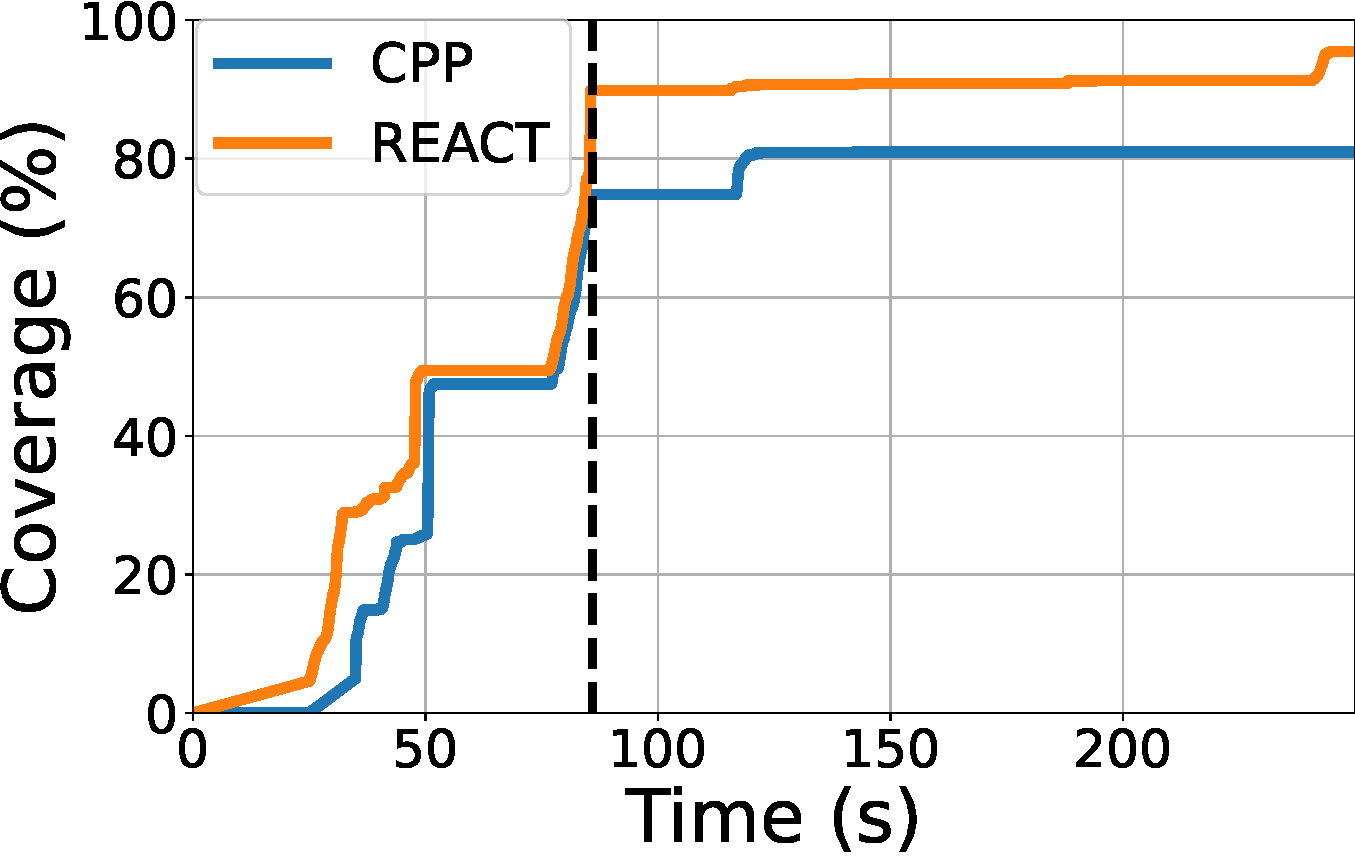
\includegraphics[width=\linewidth]{figures/dfki_coverage_comparison_plot.pdf}
        \caption{ Coverage vs. time for both planners.}
        \label{fig:traj_noreact}
    \end{subfigure}
    \hfill
    \begin{subfigure}[b]{0.44\linewidth}
        \centering
        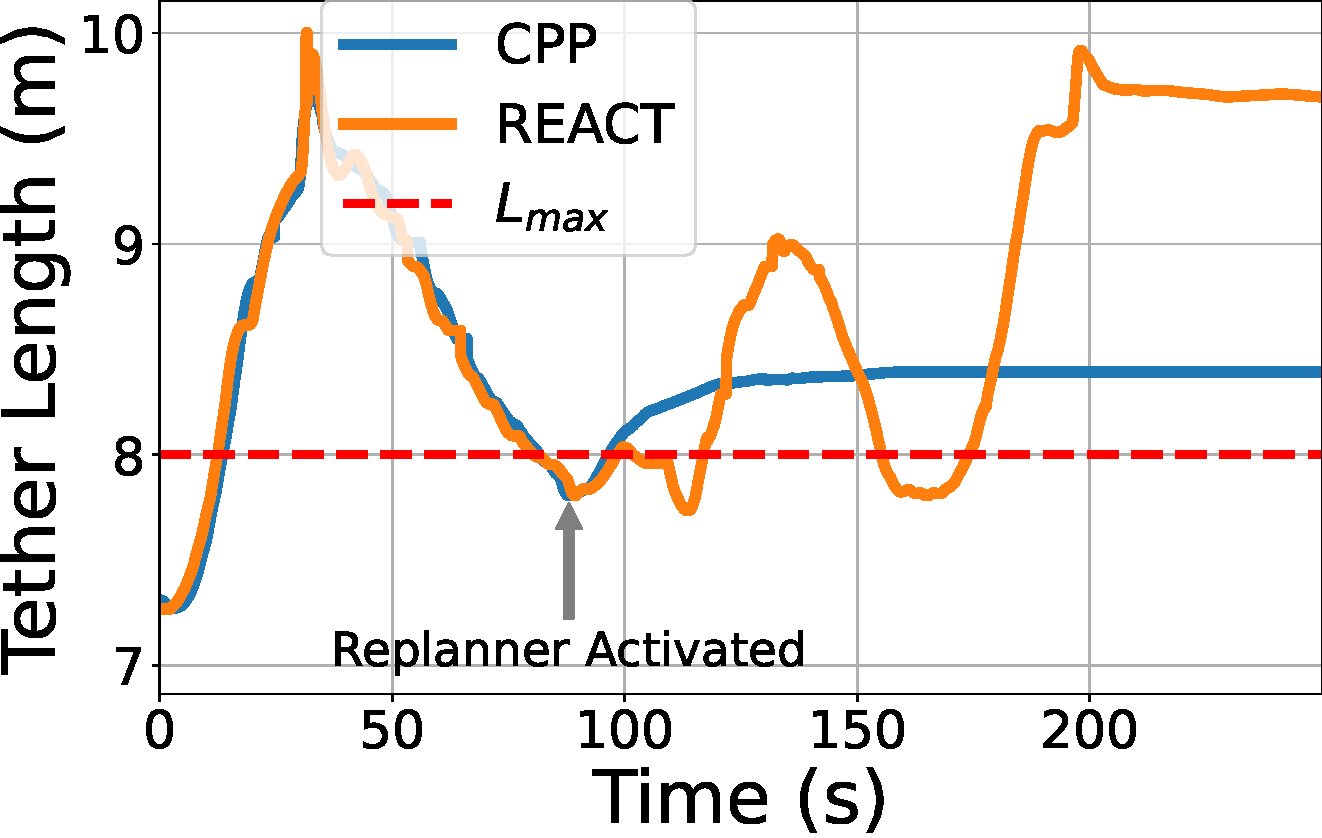
\includegraphics[width=\linewidth]{figures/dfki_tether_length_vs_time.pdf}
        \caption{Tether length vs time for both planners.}
        \label{fig:traj_react}
    \end{subfigure}
    \caption{Real-world ROV trajectories. Without \ac{REACT}, the mission fails due to tether entanglement. With \ac{REACT}, the ROV completes the mission successfully. At t = 86 s, the replanner is activated, allowing \ac{REACT} to disentangle the \ac{ROV} and continue the inspection. In contrast, at t = 124 s, the \ac{ROV} using the conventional \ac{CPP} becomes stuck due to the entangled tether.}
    \label{fig:realworld_trajectory}
\end{figure}
